\section{Design}

The PCAL has a geometry similar to the CLAS EC.  The PCAL active area is an isosceles triangle with a base length of $394$ cm and a base angle $\alpha=62.9^o$ (we will refer to the base as the back side).  The PCAL active area is slightly larger than the acceptance of the EC projected towards the CLAS target to the location of the last layer of the PCAL, see Figure \ref{pcal-triangle}. Each PCAL module is composed of 15 scintillator layers sandwiched with 14 layers of lead, similar to the inner calorimeter of the CLAS EC.  Each scintillator and lead layer is separated by a $50~\mu$m Teflon sheet and the entire scintillator/lead volume is confined within a triangular shaped box that has composite front and rear windows and aluminum side plates as shown in Figure \ref{pcal-drawing_100}. Each window consists of $2$ inch thick foam (FR-3715 Last-A-Foam, density 0.24~g~cm$^{-3}$) sandwiched between a pair of $2$ mm thick stainless steel sheets and supported by a stainless steel frame on the perimeter. Particles passing through the active area of the PCAL towards EC will pass through the forward entrance window, layers of lead and scintillator, and the rear exit window (as well as the entrance window of the EC). The full list of materials, their thicknesses and their densities are presented in Table \ref{pcal_materials}. These materials must be taken into account in the simulations. 
\begin{figure}
\centering
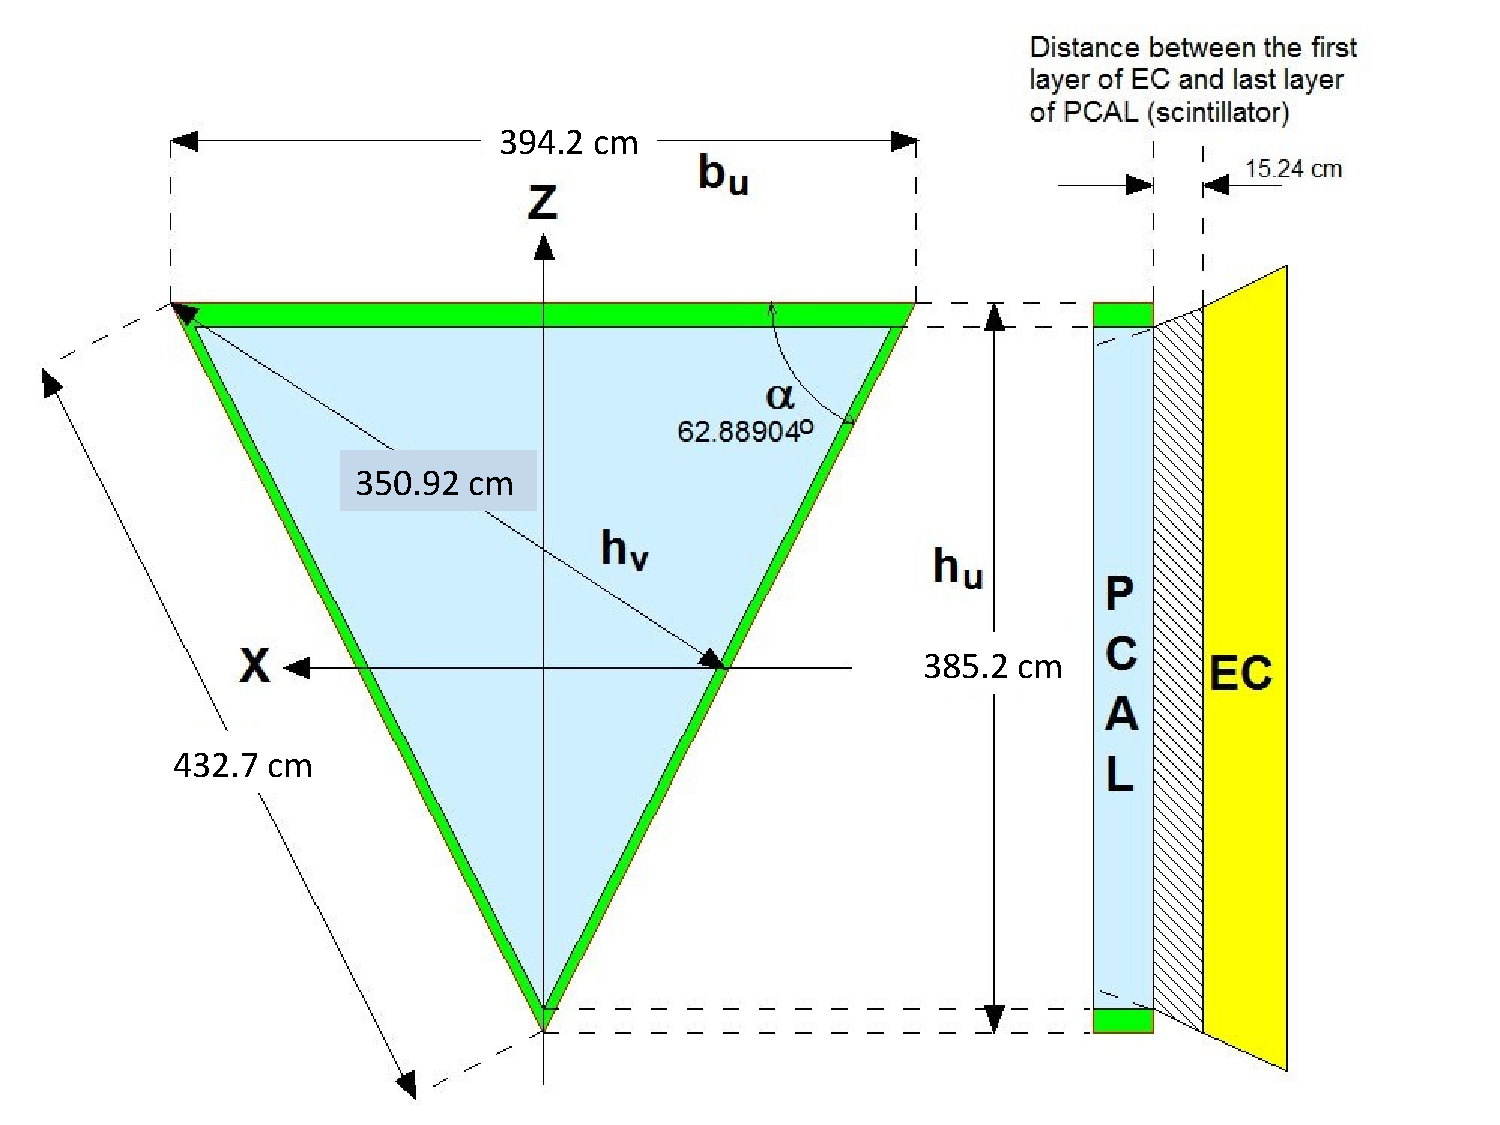
\includegraphics[scale=0.4]{pcal_ec_projection.pdf}
\caption[A schematic plot of PCAL]{A schematic plot showing the dimensions of a PCAL module. The design length $L_1$ of the longest scintillator strips are $L_1=394.2$~cm for the U strips and $L_1=432.7$~cm for the V and W strips. }
\label{pcal-triangle}
\end{figure}
All lead and scintillator layers inside the box are held in position by a retaining system attached to two of the sidewalls.  This system also allows a space between the sidewall and the end of the scintillator strips in order to route light readout fibers out of the box to the PMTs, see Figure \ref{retainers}. The scintillator layers have three alternating stereo readout planes named U, V and W. Scintillator strips of varying lengths but with a fixed cross-sectional area of $4.5 \times 1$ cm$^2$ (design values), see Figure \ref{sc-fib}, are used to construct each U, V or W readout layer. In each stereo readout layer the strips are oriented parallel to one of the sides of the triangle. For the U-view, the strips are parallel to the back side (the base of the isosceles triangle, farthest from the beamline). For the W-view, the strips are parallel to the side on which the U readout is located, the PMTs are mounted.  For the V view, the strips are parallel to the last remaining side. Light generated in the strips by ionizing radiation is transported to photomultiplier tubes (Hamamatsu R6095) mounted outside of the box via Kururay Y-11 $1$ mm diameter multi-clad wave-length shifting fibers inserted inside holes along the strips. There are $2$ holes per strip and $2$ fibers per hole are used to transport the light to the photomultiplier, see Figure \ref{sc-fib}. The readout ends of the fibers are attached to the PMTs using optical grease, the opposite ends of the fibers stick out from the far end of the strips by $\sim 1$ mm and are spot glued to the scintillator.

There are $84$ strips in the U-view, and $77$ strips in the V- and W-views. In order to optimize the number of readout channels, pair of strips at large scattering angles were combined into a single readout channel (fibers from two adjacent strips were routed to a single PMT). For the U-view only the shortest 52 strips are read out individually with a single PMT. The longest $32$ strips are paired into 16 channels, making a total of $68$ readout channels for U-redout view (see Table \ref{U-readout}.) For the V- and W-views, the $47$ longest strips are read out individually, while the $30$ shortest strips are paired into $15$ readout channels, bringing the total number of PMTs per view to $62$ (Table \ref{VW-readout}.)  The overall readout arrangement is shown in Figure \ref{readout_arrangement}. The U-strips are read out from the left-side of the triangle as seen from the target looking to the middle of the sector.  PMTs for the V- and W-views are located on the back-side of the triangle (farthest from the beamline). 

\begin{figure}
\centering
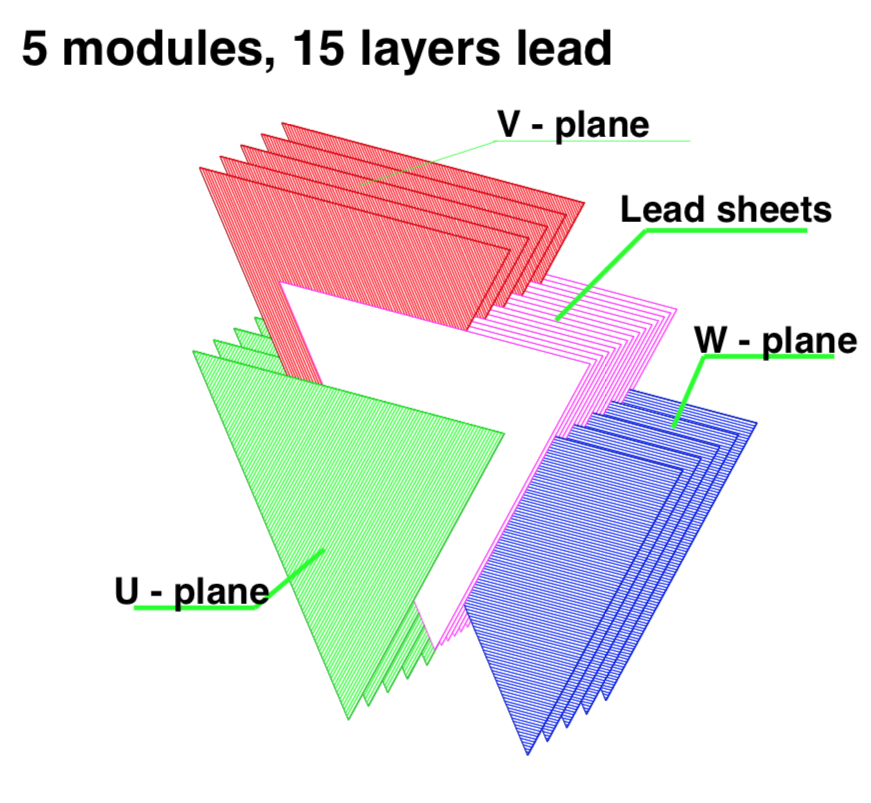
\includegraphics[scale=0.35]{pcal_layers.png}
\caption[PCAL UVW Layers]{Schematic showing interleaving of U,V,W scintillator layers with lead. }
\label{pcal-layers}
\end{figure}